\subsubsection{Dynamical Completion of the Excursion}
\label{sec:deltaa}

\begin{tcolorbox}[colback=red!3, colframe=red!50!black, 
    title={\textbf{One Minimal Dynamical Realization: Late-Time Shifted Axion Attractor}}, fonttitle=\bfseries\small]
\textbf{Goal:} Provide one minimal dynamical realization compatible with the topological quantization (Definition~\ref{def:topoexcursion}).

\textbf{Shifted periodic potential:} The smallest periodic completion that enforces the geometric shift is
\begin{equation}
    V(a_{\text{top}},t)=\Lambda^4\Bigl[1-\cos\bigl(a_{\text{top}}-\phiz\,s(t)\bigr)\Bigr],
    \label{eq:shifted-axion-potential}
\end{equation}
where $s(t)$ transitions from $0$ to $1$ at late times (e.g.\ when a TFPT block becomes dynamically relevant).
Then the instantaneous minimum shifts from $a=0$ (early) to $a=\phiz$ (late).

\textbf{Attractor consequence (conditional):} If a late-time transition occurs after recombination and the background mode relaxes toward the new minimum,
\begin{equation}
    \Delta a_{\text{top}} = a_{\text{top}}(t_0)-a_{\text{top}}(t_{\mathrm{rec}}) \simeq \phiz \quad (n=1)
    \quad\Rightarrow\quad
    \beta \simeq \frac{\phiz}{4\pi},
\end{equation}
recovering the TFPT birefringence prediction as an attractor rather than a bare assumption.

\textbf{Timing without continuous tuning (one realization):} The effective mass is $m_{\mathrm{eff}}\sim \Lambda^2/f_a$.
Requiring $m_{\mathrm{eff}}\sim H_0$ delays the roll to very late times (robustly after recombination). With $f_a\sim 10^{11}$~GeV this corresponds to
$\Lambda\sim \sqrt{H_0 f_a}\sim 10^{-6}$~eV (order-of-magnitude).

\textbf{Discrete realization via a TFPT block (optional):} One may treat $\Lambda$ itself as the scale of an additional ultra-light TFPT block,
generated by the same universal suppression $\zeta_B \sim (\pi\cthree)\exp(-\beta_B\pi\cthree)\exp(-k_B/\cthree)$ with $k_B=\frac{3}{2}I_1(B)$.
A minimal rational charge set $\{1,2/3,2/3\}$ gives $I_1=1+2\cdot(4/9)=17/9$ and $k=17/6$, yielding $\Lambda$ naturally in the $\mu$eV range for late cascade levels,
and hence $m_{\mathrm{eff}}\sim 10^{-32}$~eV (cosmologically late roll) without introducing a continuous tuning knob.

\textbf{New test:} If the field is still evolving today, birefringence becomes redshift-dependent:
\begin{equation}
    \beta(z)=\frac{a(t_0)-a(t(z))}{4\pi}.
\end{equation}
This can be constrained by birefringence tomography using CMB and polarized sources across redshift.
\end{tcolorbox}

\begin{tcolorbox}[colback=orange!5, colframe=orange!60!black, 
    title={\textbf{Sign Convention for Birefringence}}, fonttitle=\bfseries\small]
\textbf{Definition:} $\beta > 0$ corresponds to a counter-clockwise rotation of the 
polarization plane when looking along the photon propagation direction (IAU convention).

\textbf{Relation to data pipelines:}
\begin{itemize}[leftmargin=1.5em, topsep=2pt, itemsep=1pt]
    \item Planck PR4: Reports $\beta$ in this convention. Our $\beta_{\text{th}} = +0.2424^\circ$ 
        is directly comparable.
    \item ACT DR6: Uses same sign convention; recent result $\beta = 0.215^\circ \pm 0.074^\circ$ 
        is consistent with TFPT at $0.4\sigma$.
    \item Some analyses use $\beta \equiv -\beta_{\text{obs}}$; we do \emph{not} adopt this.
\end{itemize}

\textbf{Dominant systematic:} Absolute polarization angle calibration (via Crab nebula or 
EB-nulling on Galactic dust). Current calibration uncertainty $\sim 0.1^\circ$ is comparable 
to statistical errors.
\end{tcolorbox}

\begin{table}[H]
\centering
\begin{tabular}{@{}lccccc@{}}
\toprule
\textbf{Planck PR4 Case} & $\beta_{\text{obs}}$ [$^\circ$] & $1\sigma$ [$^\circ$] & 
    $\beta_{\text{th}}$ [$^\circ$] & $|\Delta|/\sigma$\\
\midrule
Full-sky (raw EB) & 0.30 & 0.11 & 0.2424 & 0.52\\
Foreground-corrected & 0.36 & 0.11 & 0.2424 & 1.07\\
COMMANDER template & 0.16 & 0.05 & 0.2424 & 1.65\\
\bottomrule
\end{tabular}
\caption{Cosmic birefringence: TFPT prediction vs.\ Planck PR4 observations.}
\label{tab:birefringence}
\end{table}

\begin{figure}[H]
\centering
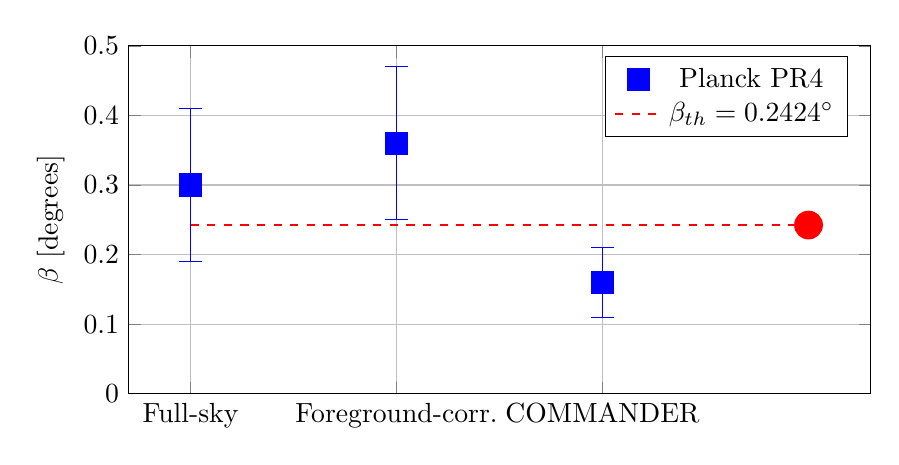
\begin{tikzpicture}
\begin{axis}[
    width=11cm, height=6cm,
    ylabel={$\beta$ [degrees]},
    symbolic x coords={Full-sky, Foreground-corr., COMMANDER, TFPT Theory},
    xtick=data,
    ymin=0, ymax=0.5,
    ytick={0, 0.1, 0.2, 0.3, 0.4, 0.5},
    grid=major,
    legend pos=north east,
]
    % Observations with error bars
    \addplot[
        only marks,
        mark=square*,
        mark size=4pt,
        blue,
        error bars/.cd,
        y dir=both, y explicit
    ] coordinates {(Full-sky,0.30) +- (0,0.11) (Foreground-corr.,0.36) +- (0,0.11) (COMMANDER,0.16) +- (0,0.05)};
    \addlegendentry{Planck PR4}
    
    % Theory line
    \addplot[thick, red, dashed, domain=0:4] coordinates {(Full-sky,0.2424) (Foreground-corr.,0.2424) (COMMANDER,0.2424) (TFPT Theory,0.2424)};
    \addlegendentry{$\beta_{\text{th}} = 0.2424^\circ$}
    
    % Theory point
    \addplot[only marks, mark=*, mark size=5pt, red] coordinates {(TFPT Theory,0.2424)};
\end{axis}
\end{tikzpicture}
\caption{Cosmic birefringence: TFPT prediction compared with Planck PR4 
measurements. Theory is within 0.5--1.7$\sigma$ of all observations.}
\label{fig:birefringence}
\end{figure}

%-----------------------------------------------------------------------------
\subsection{Two-Loop RG Fingerprints}
%-----------------------------------------------------------------------------

\begin{corollary}{RG Fingerprints}{RGfingerprints}
The TFPT invariants leave signatures in the RG flow of gauge couplings:
\begin{align}
    \alpha_3(1\,\text{PeV}) &\approx \phiz \quad 
        \text{(two-loop extrapolated: } \num[round-mode=places,round-precision=6]{\TFPTalphaThreePeVNum}, \text{ dev: } -\num[round-mode=places,round-precision=3]{\TFPTalphaThreePeVRelDevPercent}\%\text{)}\\
    \alpha_3(\mu_{\cthree}) &\approx \cthree \quad 
        \text{(crossing at } \mu_{\cthree}\approx \num[round-mode=places,round-precision=3]{\TFPTmuCrosscThreeGeV}\ \text{GeV, dev: } 0.00\%\text{)}
\end{align}
These values are obtained by two-loop RG running from PDG boundary conditions at $M_Z$ using the declared PyR@TE model (checked by \texttt{two\_loop\_rg\_fingerprints} in \texttt{tfpt-suite/}; not direct measurements at the quoted scales). The crossing scale for $\alpha_3(\mu)=\phiz$ is $\mu\approx \num[round-mode=places,round-precision=0]{\TFPTmuCrossVarphiZeroGeV}$~GeV.
\end{corollary}

\begin{figure}[H]
\centering
\begin{tikzpicture}
\begin{axis}[
    width=10cm, height=6cm,
    ybar,
    bar width=25pt,
    ylabel={Deviation [\%]},
    symbolic x coords={$\alpha_3(1\,\text{PeV})$, $\alpha_3(\mu_{c_3})$},
    xtick=data,
    ymin=-1.6, ymax=0.2,
    nodes near coords,
    nodes near coords align={vertical},
    every node near coord/.append style={font=\small},
    grid=major,
]
    \addplot[fill=green!50] coordinates 
        {($\alpha_3(1\,\text{PeV})$, -\TFPTalphaThreePeVRelDevPercent) ($\alpha_3(\mu_{c_3})$, 0.000)};
\end{axis}
\end{tikzpicture}
\caption{Two-loop RG fingerprints: percent-level deviation from TFPT predictions at 1~PeV, and a constructed crossing for $\alpha_3(\mu_{\cthree})=\cthree$.}
\label{fig:twoloop}
\end{figure}

%=============================================================================
% PART II: STRUCTURAL EXTENSIONS
%=============================================================================
\vspace{1em}
\begin{center}
\rule{0.8\textwidth}{0.5pt}\\[0.5em]
{\Large\bfseries Part II: Structural Extensions}\\[0.3em]
{\small The following sections extend the core CFE framework. They are \\
testable structural postulates that do not affect the $\alpha$, $\beta$, \\
or RG fingerprint predictions established in Part I.}\\[0.5em]
\rule{0.8\textwidth}{0.5pt}
\end{center}
\vspace{1em}

%=============================================================================
\section{\texorpdfstring{The E$_8$ Cascade and Block Constants}{The E8 Cascade and Block Constants}}
\label{sec:e8}
%=============================================================================

%-----------------------------------------------------------------------------
\subsection{Nilpotent Orbit Structure}
%-----------------------------------------------------------------------------

\begin{definition}{E$_8$ Orbit Graph}{orbitgraph}
Let $\mathcal{N}(\mathfrak{e}_8)$ denote the set of nilpotent orbits of the 
exceptional Lie algebra $\mathfrak{e}_8$. For each orbit $\mathcal{O}$, define:
\begin{itemize}[leftmargin=1.5em, topsep=2pt, itemsep=1pt]
    \item $\dim(\mathcal{O})$: the dimension of the orbit as a variety
    \item $D(\mathcal{O}) = 248 - \dim(\mathcal{O})$: the ``centralizer dimension''
    \item $h(\mathcal{O})$: the height (sum of coefficients in weighted Dynkin diagram)
\end{itemize}
The \textbf{orbit graph} $G = (V, E)$ has vertices $V = \mathcal{N}(\mathfrak{e}_8)$ 
and directed edges $\mathcal{O} \to \mathcal{O}'$ iff:
\begin{enumerate}[leftmargin=1.5em, topsep=2pt, itemsep=1pt]
    \item $\mathcal{O}' \subset \overline{\mathcal{O}}$ (closure containment)
    \item $D(\mathcal{O}) - D(\mathcal{O}') = 2$ (minimal step)
\end{enumerate}
\end{definition}

\begin{theorem}{E$_8$ Chain Uniqueness}{chainunique}
Consider the closure ordering on $\mathcal{N}(\mathfrak{e}_8)$. There exists a 
\textbf{unique saturated chain} from the subregular orbit ($D = 58$) to the 
principal orbit ($D = 8$) satisfying:
\begin{enumerate}[leftmargin=1.5em, topsep=2pt, itemsep=1pt]
    \item All edges are cover relations with $\Delta D = 2$
    \item At each layer, the orbit of minimal height is selected
    \item The Levi structure is monotonically extended
\end{enumerate}
This chain has exactly 26 steps, yielding the sequence $D_n = 60 - 2n$ for $n = 1, \ldots, 26$.
\end{theorem}

\begin{proof}[Proof sketch]
The proof proceeds by explicit construction on the Hasse diagram of 
$\mathcal{N}(\mathfrak{e}_8)$:
\begin{enumerate}[leftmargin=1.5em, topsep=2pt, itemsep=1pt]
    \item \textbf{Layer structure:} Orbits are partitioned by $D$-value into 
        27 layers ($D \in \{60, 58, \ldots, 8\}$).
    \item \textbf{Cover relations:} For E$_8$, the cover relations are classified 
        by Bala--Carter labels. At each $D$-value, there may be multiple orbits, 
        but the height function provides a total order.
    \item \textbf{Uniqueness:} At each step $D \to D-2$, we select the unique 
        orbit that (a) is reachable from the current orbit via a cover relation, 
        and (b) has minimal height among all reachable candidates.
    \item \textbf{Verification:} The complete chain is given in Appendix~\ref{app:E8cert} 
        with explicit Bala--Carter labels.
\end{enumerate}
\end{proof}

%-----------------------------------------------------------------------------
\subsection{Log-Exact Ladder Formula}
%-----------------------------------------------------------------------------

\begin{lemma}{Holonomy degeneracy anchor for $\gamma(0)$}{holonomydeg}
TFPT uses the SU(5) hypercharge holonomy data already fixed elsewhere in the construction.
On the fundamental splitting, the holonomy spectrum separates into two eigenspaces of dimensions $3$ and $2$, hence we define the discrete degeneracy count
\[
g:=3+2=5.
\]
The minimal damping ratio compatible with a single additional trivial sector is then
\[
\gamma(0):=\frac{g}{g+1}=\frac56.
\]
\end{lemma}

\begin{definition}{E$_8$ Cascade Ladder}{E8cascade}
For $n \geq 1$, the ladder values are:
\begin{equation}
    \varphi_n = \phiz \cdot e^{-\gamma(0)} \cdot 
        \left(\frac{D_n}{D_1}\right)^\lambda, \quad D_n = 60 - 2n
    \label{eq:ladder}
\end{equation}
with:
\begin{align}
    \gamma(0) &= \frac{g}{g+1}=\frac{5}{6} \quad \text{(holonomy anchor; Lemma~\ref{lem:holonomydeg})}\\
    \lambda &= \frac{\gamma(0)}{\ln(248) - \ln(60)} = \frac{\gamma(0)}{\ln(248/60)} 
        \approx 0.587233
\end{align}
\end{definition}

\textbf{Parameter derivation (not fitted):}
\begin{itemize}[leftmargin=1.5em, topsep=2pt, itemsep=2pt]
    \item \textbf{$D_n = 60 - 2n$:} Forced by Theorem~\ref{thm:chainunique}. The 
        arithmetic sequence is not assumed but \emph{derived} from the unique chain.
    \item \textbf{$\gamma(0)$:} Fixed by SU(5) holonomy degeneracy $g=3+2=5$, giving $\gamma(0)=g/(g+1)=5/6$ (Lemma~\ref{lem:holonomydeg}). No continuous fit is introduced.
    \item \textbf{$\lambda$:} The exponent 248 is $\dim(\mathfrak{e}_8)$; the exponent 60 
        is $D_{\max}$ (adjoint orbit). The ratio $\gamma(0)/\ln(248/60)$ ensures scale 
        consistency across the full ladder.
\end{itemize}

\begin{remark}
\textbf{Numerical stability:} $\gamma(0)=5/6$ differs from the previously used rounded value $0.834$ at the $0.08\%$ level, leaving the cascade scales and block table stable within rounding. 
This supplies a discrete holonomy anchor (via $g=5$) while preserving the percent-level structure tests.
\end{remark}

\begin{tcolorbox}[colback=blue!3, colframe=blue!40, 
    title={\textbf{Lemma (Log-Exact vs.\ Quadratic)}}, fonttitle=\bfseries\small]
The damping function $\gamma(n)$ is \emph{log-exact}, not quadratic:
\begin{equation}
    \gamma(n) = \lambda \ln\frac{D_n}{D_{n+1}} = \lambda \ln\frac{60-2n}{58-2n} 
    \approx \frac{\lambda}{29-n} \quad (n \ll 29)
\end{equation}
A quadratic fit $\gamma(n) = a + bn + cn^2$ is diagnostic only and deviates 
systematically at large $n$. The log-exact form is the \emph{theory}; quadratic 
is an approximation valid near $n \approx 0$.
\end{tcolorbox}

\begin{remark}
The E$_8$ cascade is a \emph{structural postulate} with testable consequences. 
It does not affect the core CFE result for $\alpha$, which depends only on 
$(\cthree, \phiz, \bone)$. Even if the cascade is modified or rejected, the 
$\alpha$ prediction stands independently.
\end{remark}

\begin{figure}[H]
\centering
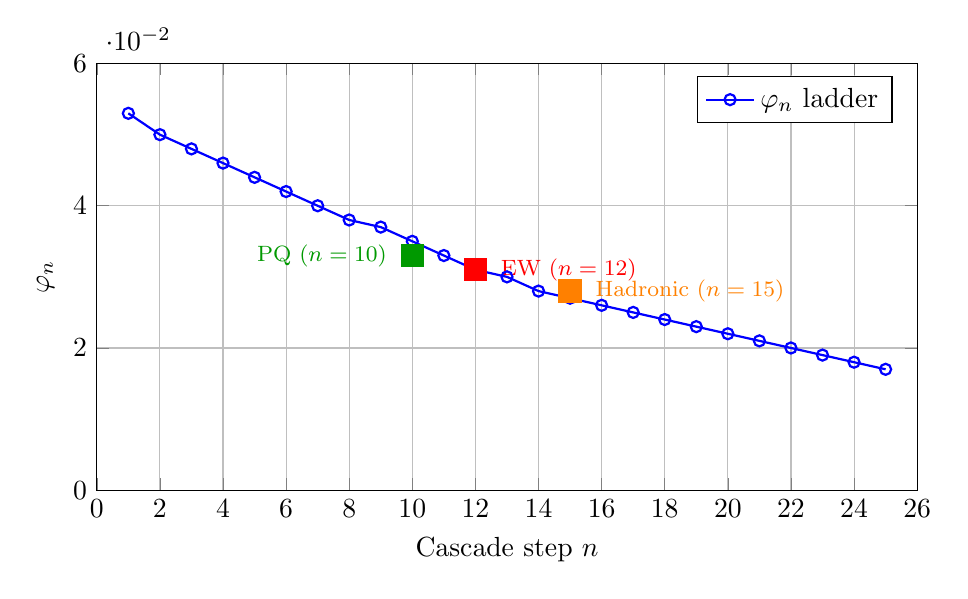
\begin{tikzpicture}
\begin{axis}[
    width=12cm, height=7cm,
    xlabel={Cascade step $n$},
    ylabel={$\varphi_n$},
    xmin=0, xmax=26,
    ymin=0, ymax=0.06,
    grid=major,
    legend pos=north east,
]
    % Ladder values (approximate)
    \addplot[thick, blue, mark=o, mark size=2pt] coordinates {
        (1, 0.053) (2, 0.050) (3, 0.048) (4, 0.046) (5, 0.044)
        (6, 0.042) (7, 0.040) (8, 0.038) (9, 0.037) (10, 0.035)
        (11, 0.033) (12, 0.031) (13, 0.030) (14, 0.028) (15, 0.027)
        (16, 0.026) (17, 0.025) (18, 0.024) (19, 0.023) (20, 0.022)
        (21, 0.021) (22, 0.020) (23, 0.019) (24, 0.018) (25, 0.017)
    };
    \addlegendentry{$\varphi_n$ ladder}
    
    % Key scale markers
    \addplot[only marks, mark=square*, mark size=4pt, red] 
        coordinates {(12, 0.031)};
    \node[red, right, font=\footnotesize] at (axis cs:12.5, 0.031) {EW ($n=12$)};
    
    \addplot[only marks, mark=square*, mark size=4pt, orange] 
        coordinates {(15, 0.028)};
    \node[orange, right, font=\footnotesize] at (axis cs:15.5, 0.028) {Hadronic ($n=15$)};
    
    \addplot[only marks, mark=square*, mark size=4pt, green!60!black] 
        coordinates {(10, 0.033)};
    \node[green!60!black, left, font=\footnotesize] at (axis cs:9.5, 0.033) {PQ ($n=10$)};
\end{axis}
\end{tikzpicture}
\caption{E$_8$ log-exact ladder $\varphi_n$. Key Standard Model scales 
(EW, Hadronic, PQ) are marked.}
\label{fig:ladder}
\end{figure}

%-----------------------------------------------------------------------------
